\documentclass[10pt]{beamer}

\usetheme[progressbar=frametitle]{metropolis}
\usepackage{appendixnumberbeamer}
\usepackage{graphicx}
\usepackage{caption}
\usepackage{subcaption}
\usepackage{booktabs}
\usepackage[scale=2]{ccicons}

\usepackage{pgfplots}
\usepgfplotslibrary{dateplot}
\usepackage[sorting=none]{biblatex}
\addbibresource{9th_sem_presentation/presentation_ref.bib}
\usepackage{xspace}
\newcommand{\themename}{\textbf{\textsc{metropolis}}\xspace}
% --- your physics packages (from last answer) ---
\usepackage{amsmath,amssymb,amsthm}
\usepackage{bm}
\usepackage{physics}
\usepackage{braket}
\usepackage{mathtools}
\usepackage{siunitx}
\usepackage{cancel}
\usepackage{physics}
% In preamble
\newcommand{\slidecitation}[1]{%
  \vfill
  \begin{flushright}
    \scriptsize #1
  \end{flushright}
}

\usepackage{tikz}
\usetikzlibrary{arrows.meta,positioning,calc,decorations.pathmorphing,shapes,fit}
\tikzset{
  spin/.style={circle,draw,inner sep=1pt,minimum size=7mm,font=\small},
  fliparrow/.style={->, thick, color=blue}
}


\title{Hilbert space fragmentation in Floquet-driven systems}
\subtitle{Ninth-semester presentation}
% \date{\today}
\date{}
\author{Rishi Paresh Joshi\\Under the guidance of Dr Tapan Mishra}
\institute{National Institute of Science Education and Research}
% \titlegraphic{\hfill\includegraphics[height=1.5cm]{logo.pdf}}

\begin{document}

\maketitle

\begin{frame}{Table of contents}
  \setbeamertemplate{section in toc}[sections numbered]
  \tableofcontents%[hideallsubsections]
\end{frame}

\section{Out-of-equilibrium quantum dynamics}

\begin{frame}{Equilibrium dynamics}
  \begin{itemize}
    \item Equilibrium: ensembles, defined by conserved quantities
    \item Isolated, time-independent Hamiltonian, $H$
    \item Microcanonical description is on an energy shell
    \item In most ergodic systems $\Rightarrow$ Eigenstate thermalisation hypothesis (ETH) is satisfied
    \item The microcanonical density matrix is
  \end{itemize}

  \vspace{0.4cm}
  \[
    \rho_{\mathrm{mc}} \propto
    \sum_{E_n \in [E,E+\Delta E]} \ket{n}\bra{n}
  \]

\begin{center}
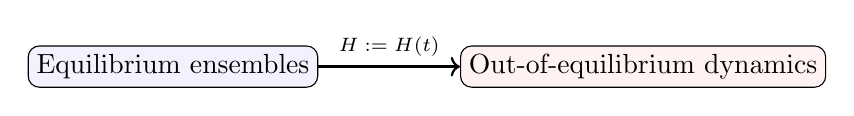
\begin{tikzpicture}
  % equilibrium box
  \node[draw, rounded corners, fill=blue!5, inner sep=3pt] (eq) {Equilibrium ensembles};

  % out-of-equilibrium box
  \node[draw, rounded corners, fill=red!5, inner sep=3pt, right=1.8cm of eq] (ne) {Out-of-equilibrium dynamics};

  % arrow
  \draw[->, thick] (eq) -- node[above, font=\scriptsize] { $H:=H(t)$} (ne);
\end{tikzpicture}
\end{center}



\end{frame}

% ------------------------------------------------

\begin{frame}{Quenches, ramps, and general drives}
Different types of time dependent Hamiltonians are studied in physics:
  \begin{columns}[T,onlytextwidth]
    \column{0.55\textwidth}
      \begin{itemize}
        \item Quantum quench: $H_{\mathrm{i}} \to H_{\mathrm{f}}$ at some time
        \item Ramp / slow quench: \\control parameter \\$\lambda(t)$
        varies very slowly
        \item General drive: continuously varying time dependence
      \end{itemize}
Thus, in general:
      \[
        H(t) = H[\lambda(t)]
      \]
      

    \column{0.45\textwidth}
 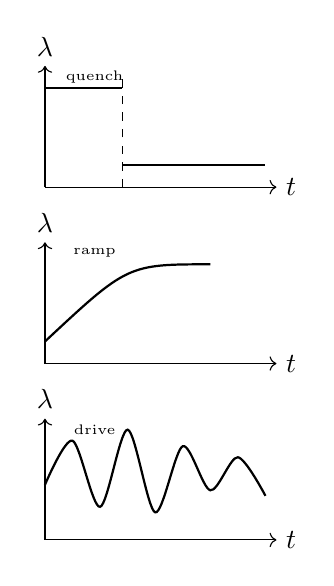
\begin{tikzpicture}[scale=0.7]
  % axes
  \draw[->] (0,0) -- (4.2,0) node[right] {$t$};
  \draw[->] (0,0) -- (0,2.2) node[above] {$\lambda$};

  % quench
  \draw[thick] (0,1.8) -- (1.4,1.8);
  \draw[thick] (1.4,0.4) -- (4,0.4);
  \draw[dashed] (1.4,0) -- (1.4,2.0);
  \node[font=\tiny] at (0.9,2.0) {quench};

  % ramp
  \begin{scope}[yshift=-3.2cm] % << increased spacing
    \draw[->] (0,0) -- (4.2,0) node[right] {$t$};
    \draw[->] (0,0) -- (0,2.2) node[above] {$\lambda$};
    \draw[thick] (0,0.4) .. controls (1.5,1.8) .. (3,1.8);
    \node[font=\tiny] at (0.9,2.0) {ramp};
  \end{scope}

  % wiggly drive
  \begin{scope}[yshift=-6.4cm] % << increased spacing
    \draw[->] (0,0) -- (4.2,0) node[right] {$t$};
    \draw[->] (0,0) -- (0,2.2) node[above] {$\lambda$};
    \draw[thick,smooth] plot coordinates {
      (0,1.0) (0.5,1.8) (1,0.6) (1.5,2.0)
      (2,0.5) (2.5,1.7) (3,0.9) (3.5,1.5) (4,0.8)
    };
    \node[font=\tiny] at (0.9,2.0) {drive};
  \end{scope}
\end{tikzpicture}

  \end{columns}
\end{frame}

% ------------------------------------------------

\begin{frame}{Periodically driven (Floquet) systems}
  \begin{columns}[T,onlytextwidth]
    \column{0.55\textwidth}
      \begin{itemize}
        \item Special case: periodic drive
        \item Hamiltonian repeats with period $T$
        \item Focus on evolution over one period
        \item Stroboscopic times: $t = nT$
      \end{itemize}

      \[
        H(t+T) = H(t)
      \]

      \[
        U_F = \mathcal{T}
        \exp\!\left(-i\int_{0}^{T} H(t)\,dt\right)
      \]

    \column{0.45\textwidth}
      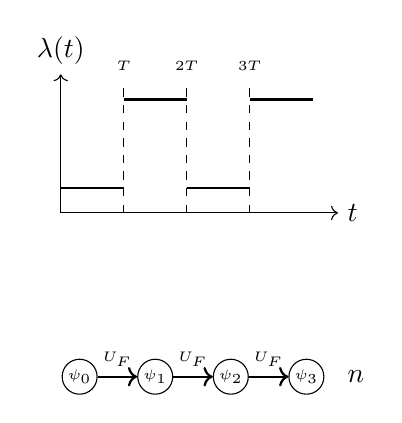
\begin{tikzpicture}[scale=0.8]
        % J(t) periodic
        \draw[->] (0,0) -- (4.4,0) node[right] {$t$};
        \draw[->] (0,0) -- (0,2.2) node[above] {$\lambda(t)$};

        \draw[thick] (0,0.4) -- (1,0.4);
        \draw[thick] (1,1.8) -- (2,1.8);
        \draw[thick] (2,0.4) -- (3,0.4);
        \draw[thick] (3,1.8) -- (4,1.8);

        \draw[dashed] (1,0) -- (1,2.1) node[above, font=\tiny] {$T$};
        \draw[dashed] (2,0) -- (2,2.1) node[above, font=\tiny] {$2T$};
        \draw[dashed] (3,0) -- (3,2.1) node[above, font=\tiny] {$3T$};

        % stroboscopic chain
        \begin{scope}[yshift=-2.6cm]
  % Remove or comment out the axis arrow:
  % \draw[->] (0,0) -- (4.4,0) node[right] {$n$};
  \node[circle,draw,inner sep=1pt,font=\tiny] (p0) at (0.3,0) {$\psi_0$};
  \node[circle,draw,inner sep=1pt,font=\tiny] (p1) at (1.5,0) {$\psi_1$};
  \node[circle,draw,inner sep=1pt,font=\tiny] (p2) at (2.7,0) {$\psi_2$};
  \node[circle,draw,inner sep=1pt,font=\tiny] (p3) at (3.9,0) {$\psi_3$};

  \draw[->,thick] (p0) -- node[above, font=\tiny] {$U_F$} (p1);
  \draw[->,thick] (p1) -- node[above, font=\tiny] {$U_F$} (p2);
  \draw[->,thick] (p2) -- node[above, font=\tiny] {$U_F$} (p3);
  \node[right] at (4.4,0) {$n$};

\end{scope}

      \end{tikzpicture}
  \end{columns}
\end{frame}
\section{Eigenstate thermalization}
\begin{frame}{Eigenstate thermalisation hypothesis: why naive time averaging is not enough}
\begin{columns}[T,onlytextwidth]

\column{0.55\textwidth}
\small
\begin{itemize}
  \item Closed quantum system
  \item Energy basis: $\ket{\psi(0)}=\sum_m C_m \ket{E_m}$
  \item Few-body observable $A$; persistent oscillations\\ $\langle A\rangle(t)= \sum_n p_n A_{nn}
   + \sum_{m\neq n} c_m^\ast c_n e^{i(E_m-E_n)t}A_{mn}$
  \item Ces\`aro long-time average (diagonal ensemble):
  \[
    \overline{\langle A\rangle}
    = \lim_{T\to\infty}\frac{1}{T}
      \int_0^T \langle A\rangle(t)\,dt
    = \sum_m |C_m|^2 A_{mm}
  \]
  \item Problems: Heisenberg time$\sim e^{cL}$, Initial conditions preserved ;
\end{itemize}


\column{0.45\textwidth}
\centering
\begin{figure}
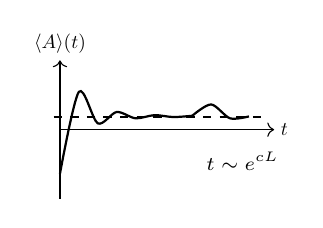
\begin{tikzpicture}[scale=0.8]
  % axes
  \draw[->] (0,0) -- (3.4,0) node[right,scale=0.7] {$t$};
  \draw[->] (0,-1.1) -- (0,1.1) node[above,scale=0.7] {$\langle A\rangle(t)$};

  % fast relaxation
  \draw[thick,smooth]
    plot coordinates {
      (0,-0.7) (0.3,0.6) (0.6,0.1)
      (0.9,0.28) (1.2,0.18) (1.5,0.23)
      (1.8,0.2) (2.1,0.22)
    };

  % tiny late revival bump
  \draw[thick,smooth]
    plot coordinates {
      (2.1,0.22) (2.4,0.4) (2.7,0.18) (3.0,0.21)
    };

  % plateau
  \draw[dashed] (-0.1,0.2) -- (3.2,0.2);

  % labels
    \node[font=\scriptsize] at (2.9,-0.5) {$t\sim e^{cL}$};
\end{tikzpicture}
\end{figure}
\begin{figure}
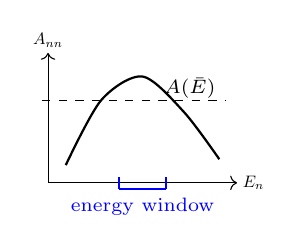
\begin{tikzpicture}[scale=0.75]

  % axes
  \draw[->] (0,0) -- (3.2,0) node[right,scale=0.6] {$E_n$};
  \draw[->] (0,0) -- (0,2.2) node[above,scale=0.6] {$A_{nn}$};

  % smooth curve
  \draw[thick,smooth]
    plot coordinates {
      (0.3,0.3) (0.9,1.4)
      (1.6,1.8) (2.3,1.2) (2.9,0.4)
    };

  % microcanonical window
  \draw[thick,blue] (1.2,-0.1) -- (2.0,-0.1);
  \draw[thick,blue] (1.2,-0.1) -- (1.2,0.1);
  \draw[thick,blue] (2.0,-0.1) -- (2.0,0.1);
  \node[font=\scriptsize,blue] at (1.6,-0.4) {energy window};

  % horizontal line at A(Ebar)
  \draw[dashed] (-0.1,1.4) -- (3.0,1.4);
  \node[font=\scriptsize] at (2.4,1.6) {$A(\bar E)$};

\end{tikzpicture}
\end{figure}
\end{columns}
\slidecitation{L.~D'Alessio, Y.~Kafri, A.~Polkovnikov, and M.~Rigol,
``From quantum chaos and eigenstate thermalization to statistical mechanics and
thermodynamics'', \textit{Advances in Physics} (2016).}
\end{frame}
%========= RMT SLIDE 1 =========
\begin{frame}{Eigenstate thermalisation}

\small
\begin{columns}[T,onlytextwidth]

\column{0.45\textwidth}
\begin{itemize}\setlength\itemsep{3pt}
  \item Chaotic eigenstates take random directions in Hilbert space
  \item Any local operator, $\textbf{A}$ is diagonal in product basis but scrambled in energy basis
  \item Diagonal elements of  $\textbf{A}$ vary smoothly versus energy as energy eigenstates are thermal
  \item Off-diagonals decay exponentially with size and are controlled by temporal fluctuations
  \item $\textbf{A}$ relaxes to plateau given by the ensemble average
\end{itemize}

\column{0.55\textwidth}
\centering
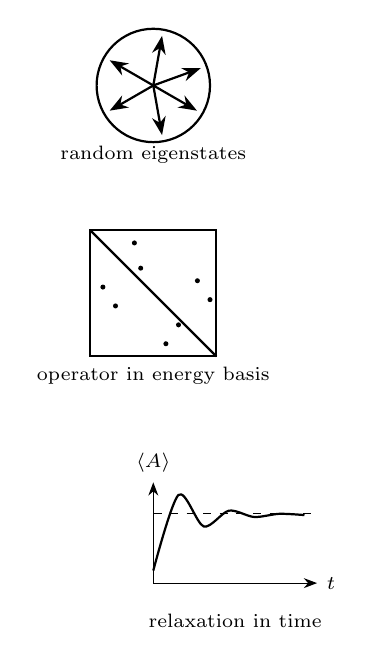
\begin{tikzpicture}[scale=0.8,>=Stealth]

  % Panel 1: random eigenstates
  \begin{scope}[yshift=2.6cm]
    \draw[thick] (0,0) circle (0.9);
    \foreach \ang in {20,80,150,210,280,330} {
      \draw[->,thick] (0,0) -- ({0.8*cos(\ang)},{0.8*sin(\ang)});
    }
    \node[font=\scriptsize,align=center] at (0,-1.1)
      {random eigenstates};
  \end{scope}

  % Panel 2: operator matrix in energy basis
  \begin{scope}[yshift=-0.7cm]
    \draw[thick] (-1,-1) rectangle (1,1);
    \draw[line width=0.8pt] (-1,1) -- (1,-1);
    \foreach \x/\y in {
      -0.6/-0.2, -0.2/0.4, 0.4/-0.5, 0.7/0.2,
      -0.3/0.8, 0.2/-0.8, -0.8/0.1, 0.9/-0.1
    }{
      \fill (\x,\y) circle (0.04);
    }
    \node[font=\scriptsize,align=center] at (0,-1.3)
      {operator in energy basis};
  \end{scope}

  % Panel 3: relaxation in time
  \begin{scope}[yshift=-5.3cm]
    \draw[->] (0,0) -- (2.6,0) node[right,font=\scriptsize] {$t$};
    \draw[->] (0,0) -- (0,1.6) node[above,font=\scriptsize] {$\langle A\rangle$};
    \draw[dashed] (0,1.1) -- (2.6,1.1);
    \draw[thick,smooth] plot coordinates {
      (0,0.2) (0.4,1.4) (0.8,0.9)
      (1.2,1.15) (1.6,1.05) (2.0,1.1) (2.4,1.08)
    };
    \node[font=\scriptsize,align=center] at (1.3,-0.6)
      {relaxation in time};
  \end{scope}

\end{tikzpicture}

\end{columns}
\slidecitation{M.~Srednicki, ``Chaos and Quantum Thermalization", Phys.\ Rev.\ E 50, 888 (1994)} 
\end{frame}



%==================== ETH SLIDE 3 ====================



%==================== ETH SLIDE 4 ====================



%==================== ETH SLIDE 5 ====================



%==================== ETH SLIDE 6 ====================

\begin{frame}{ETH in Floquet heating}

\begin{columns}[T,onlytextwidth]

\column{0.55\textwidth}
\small
\begin{itemize}
  \item Periodic drive:
        $H(t+T)=H(t)$
  \item Floquet unitary:
        $U_F=\mathcal{T}\exp\!\bigl(-i\int_0^T H(t)\,dt\bigr)$
  \item Effective Floquet Hamiltonian:
        $U_F=e^{-iH_F T}$
  \item Energy not conserved;
        only symmetries of $U_F$ (e.g.\ total $S^z$)
  \item ETH for $H_F$ in \textbf{global} symmetry sector $\mathcal{S}$:
        eigenstates $\ket{\phi_\alpha}$ locally random in $\mathcal{S}$
  \item Diagonal Floquet ETH:
  \[
    \matrixel{\phi_\alpha}{A}{\phi_\alpha}
    \approx \frac{1}{\dim\mathcal{S}}\Tr_{\mathcal{S}} A
  \]

\end{itemize}

\column{0.45\textwidth}
\centering
\begin{figure}
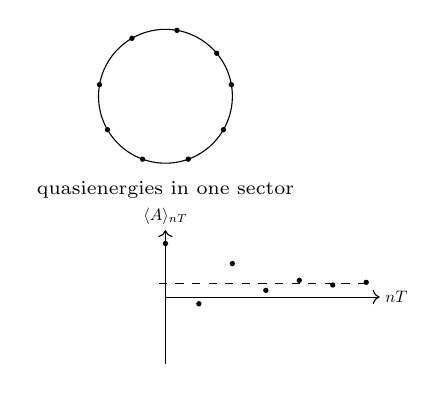
\begin{tikzpicture}[scale=0.85]

  % quasienergy circle
  \draw (0,0) circle (1.0);
  \foreach \ang in {10,40,80,120,170,210,250,290,330} {
    \fill ({cos(\ang)},{sin(\ang)}) circle (0.04);
  }
  \node[font=\scriptsize] at (0,-1.4) {quasienergies in one sector};

  % time evolution of <A> at nT
  \begin{scope}[xshift=0.0cm,yshift=-3cm]
    \draw[->] (0,0) -- (3.2,0) node[right,scale=0.6] {$nT$};
    \draw[->] (0,-1.0) -- (0,1.0) node[above,scale=0.6] {$\langle A\rangle_{nT}$};
    \draw[dashed] (-0.1,0.2) -- (3.1,0.2);

    \foreach \n/\y in {0/0.8, 0.5/-0.1, 1.0/0.5, 1.5/0.1, 2.0/0.25, 2.5/0.18, 3.0/0.22} {
      \fill (\n,\y) circle (0.04);
    }
  \end{scope}

\end{tikzpicture}

\end{figure}
\slidecitation{L.~D'Alessio and M.~Rigol,
``Long-time behavior of isolated periodically driven interacting lattice systems'',
\textit{Physical Review X} (2014).}

\end{columns}
Floquet heating is when local observables take infinite-temperature values in $\mathcal{S}$ (they become random)
\end{frame}

%============== PART 3 – SLIDE 1 ==============


\section{Violation of eigenstate thermalisation through Hilbert space fragmentation}
%============== PART 3 – SLIDE 2 ==============
\begin{frame}{Avoiding Floquet heating: ETH-violating mechanisms}

\begin{columns}[T,onlytextwidth]

\column{0.55\textwidth}
\small
\begin{itemize}
  \item ETH is robust but not universal
  \item Integrability: The presence of a large number of conserved quantities leads to loss of ergodicity and prevents the realisation of long-time thermal steady states.
  \item MBL: The system becomes non-ergodic due to strong disorder, leading to localisation of all states in its Hilbert space.
  \item Scars: special nonthermal eigenstates;
        long-time oscillations
  \item Fragmentation: local constraints;\\
        many disconnected Krylov sectors
\end{itemize}

\column{0.45\textwidth}
\centering
\begin{figure}
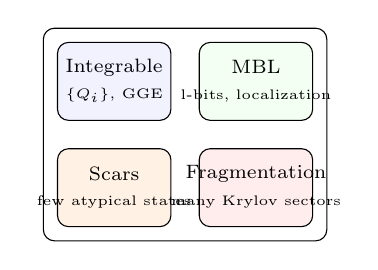
\begin{tikzpicture}[scale=0.9]
  % big box
  \draw[rounded corners] (0,0) rectangle (4,3);

  % four mechanism boxes
  \draw[rounded corners,fill=blue!5] (0.2,1.7) rectangle (1.8,2.8);
  \node[font=\scriptsize] at (1.0,2.45) {Integrable};
  \node[font=\tiny] at (1.0,2.05) {$\{Q_i\}$, GGE};

  \draw[rounded corners,fill=green!5] (2.2,1.7) rectangle (3.8,2.8);
  \node[font=\scriptsize] at (3.0,2.45) {MBL};
  \node[font=\tiny] at (3.0,2.05) {l-bits, localization};

  \draw[rounded corners,fill=orange!10] (0.2,0.2) rectangle (1.8,1.3);
  \node[font=\scriptsize] at (1.0,0.95) {Scars};
  \node[font=\tiny] at (1.0,0.55) {few atypical states};

  \draw[rounded corners,fill=red!7] (2.2,0.2) rectangle (3.8,1.3);
  \node[font=\scriptsize] at (3.0,0.95) {Fragmentation};
  \node[font=\tiny] at (3.0,0.55) {many Krylov sectors};

\end{tikzpicture}
\end{figure}
\slidecitation{D.~A.~Abanin, E.~Altman, I.~Bloch, and M.~Serbyn,
``Colloquium: Many-body localization, thermalization, and entanglement'',
\textit{Reviews of Modern Physics} (2019);\,
R.~Nandkishore and D.~A.~Huse,
``Many-Body Localization and Thermalization in Quantum Statistical Mechanics'',
\textit{Annual Review of Condensed Matter Physics} (2015).}

\end{columns}
 Floquet prethermal fragmentation: restricted exploration of Hilbert space; slowed or prevented heating due to fragmentation in first order Floquet Hamiltonian
\end{frame}

\begin{frame}{Hilbert space fragmentation (HSF): static picture}

\begin{columns}[T,onlytextwidth]

\column{0.55\textwidth}
\small
\begin{itemize}
  \item Family of Hilbert spaces $\mathcal{H}(L)$;\\
        $\dim\mathcal{H}(L)\sim e^{cL}$
  \item Fragmented operator $X(L)$:
  \[
    \mathcal{H}(L)
    = \bigoplus_{\alpha=1}^{N_{\mathrm{frag}}(L)}
      \mathcal{K}_\alpha(L)
  \]
  \item Invariance:
        $X(L)\,\mathcal{K}_\alpha(L)\subseteq\mathcal{K}_\alpha(L)$
  \item Strong fragmentation:
        $N_{\mathrm{frag}}(L)\sim e^{s_{\mathrm{frag}}L}$
  \item Typical fragments:
        $\dim\mathcal{K}_\alpha(L)\ll\dim\mathcal{H}(L)$
  \item Result: eigenstates in tiny islands;\\
        ETH only inside $\mathcal{K}_\alpha$,\\
        strong ergodicity breaking
\end{itemize}

\column{0.45\textwidth}
\begin{figure}
    \centering
    \includegraphics[width=1\linewidth]{9th_sem_presentation/HSF blocks.png}
    
    \label{HSF blocks}
\end{figure}



\begin{figure}
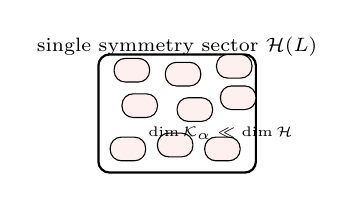
\begin{tikzpicture}[scale=0.5]

  % big symmetry sector
  \draw[rounded corners,thick] (0,0) rectangle (4,3);
  \node[font=\scriptsize] at (2,3.2) {single symmetry sector $\mathcal{H}(L)$};

  % many small fragments
  \foreach \x/\y in {0.3/0.3,1.5/0.4,2.7/0.3,0.6/1.4,2.0/1.3,3.1/1.6,0.4/2.3,1.7/2.2,3.0/2.4} {
    \draw[rounded corners,fill=red!6] (\x,\y) rectangle ++(0.9,0.6);
  }

  \node[font=\tiny] at (3.1,1.0) {$\dim\mathcal{K}_\alpha\ll\dim\mathcal{H}$};

\end{tikzpicture}
\end{figure}


\end{columns}
\slidecitation{S.~Moudgalya and O.~I.~Motrunich,
``Hilbert Space Fragmentation and Commutant Algebras'',
\textit{Physical Review X} (2022).}

\end{frame}
\begin{frame}{Example of HSF in static system}
   

    \vspace{-0.3cm}
    \small
    \begin{itemize}
      \item Spin-1 chain with three-site dipole-conserving Hamiltonian\\
    $H_3 = -\sum_n \big[ S_n^+ (S_{n+1}^-)^2 S_{n+2}^+ + \text{H.c.} \big], H_4 = -\sum_n [S_n^+ S_{n+1}^- S_{n+2}^- S_{n+3}^+ + H.c.]$
      \item Global conserved quantities: charge and dipole moment $Q = \sum_n S_n^z$, \quad $P = \sum_n n S_n^z$
      \item Explore autocorrelation: $C_j^z(t) \equiv \langle S_j^z(t) S_j^z(0) \rangle$
      \item Finite long-time plateau of $C_0^z(t)$ at infinite temperature $\Rightarrow$ persistent local memory, weak ETH violation-strong HSF ($H_3$). 
    \end{itemize}

 \begin{figure}
        \centering
        \includegraphics[width=0.7\linewidth]{9th_sem_presentation/PabloSalaAutocorrelation.png}
        \label{PabloSalaAutocorrelation}
    \end{figure}
\slidecitation{P.~Sala, T.~Rakovszky, R.~Verresen, M.~Knap, and F.~Pollmann,
``Ergodicity Breaking Arising from Hilbert Space Fragmentation in Dipole-Conserving Hamiltonians'',
\textit{Physical Review X} (2020).}

\end{frame}

%============== PART 3 – SLIDE 3 ==============


\begin{frame}{Hilbert space fragmentation in driven system}
\begin{columns}[T,onlytextwidth]

\column{0.55\textwidth}
\small
\begin{itemize}
  \item Fragmentation inherited by the Floquet unitary and projector operator, $P_\alpha$:
  \[
    U_F = \bigoplus_\alpha U_F^{(\alpha)},\qquad
    [U_F,P_\alpha]=0
  \]
  \item Stroboscopic dynamics:
        $\ket{\psi(0)}\in\mathcal{K}_\alpha
        \Rightarrow \ket{\psi(nT)}\in\mathcal{K}_\alpha$
  \item Fragment-restricted infinite-$T$ ensemble:
  \[
    \rho_\infty^{(\alpha)}
    = \frac{P_\alpha}{\dim\mathcal{K}_\alpha}
  \]
  \item ETH inside fragment only;\\
        $\overline{\langle A\rangle}_\alpha
        \approx \frac{1}{\dim\mathcal{K}_\alpha}\Tr(P_\alpha A)$

\end{itemize}

\column{0.45\textwidth}
\centering
\begin{figure}
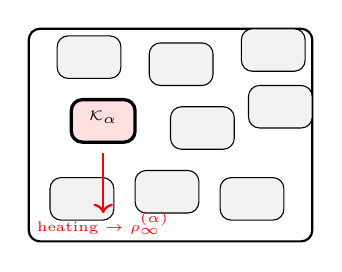
\begin{tikzpicture}[scale=0.9]

  % big box
  \draw[rounded corners,thick] (0,0) rectangle (4,3);

  % many fragments (faint)
  \foreach \x/\y in {0.3/0.3,1.5/0.4,2.7/0.3,0.6/1.4,2.0/1.3,3.1/1.6,0.4/2.3,1.7/2.2,3.0/2.4} {
    \draw[rounded corners,fill=gray!10] (\x,\y) rectangle ++(0.9,0.6);
  }

  % highlighted active fragment
  \draw[rounded corners,very thick,fill=red!12] (0.6,1.4) rectangle ++(0.9,0.6);
  \node[font=\tiny] at (1.05,1.75) {$\mathcal{K}_\alpha$};

  % arrow indicating heating inside fragment
  \draw[->,thick,red] (1.05,1.25) -- (1.05,0.4);
  \node[font=\tiny,red] at (1.05,0.25) {heating $\rightarrow$ $\rho_\infty^{(\alpha)}$};

\end{tikzpicture}
\end{figure}
\slidecitation{S.~Ghosh, I.~Paul, and K.~Sengupta,
``Prethermal Fragmentation in a Periodically Driven Fermionic Chain'',
\textit{Physical Review Letters} (2023).}
.
\end{columns}

\end{frame}
\begin{frame}{Example of prethermal HSF in driven system: Model}


  \vspace{-1ex}
  \small
  Hamiltonian given by $H(t) = H_0(t) + H_1$,
$$H_0(t) = V(t) \sum_{j=1..L} \hat{n}_j\hat{n}_{j+1}$$
$$H_1 = \sum_{j=1..L} -J(c_j^\dagger c_{j+1} + H.c.) + \hat{n}_j(V_0\hat{n}_{j+1} + V_2\hat{n}_{j+2}),$$
 Periodic drive of NN interaction: $V(t) = 
\begin{cases}
- V_1, & t \leq \dfrac{T}{2} \\
+ V_1, & t > \dfrac{T}{2}
\end{cases}$; high-frequency regime, First-order Floquet Hamiltonian $H_F^{(1)}$ from Floquet perturbation theory

  $
    H_F^{(1)} =
    \sum_j \hat n_j (V_0 \hat n_{j+1} + V_2 \hat n_{j+2})
    - J \sum_j \Bigl[(1-\hat A_j^2)+ f(\gamma_0)\,\hat A_j^2\Bigr]
      (c_j^\dagger c_{j+1} + \text{h.c.})
  $
  \[
    \hat A_j = \hat n_{j+2}-\hat n_{j-1},\qquad
    \gamma_0 = \frac{V_1 T}{4\hbar},\qquad
    f(\gamma_0)=0 \ \text{at special } \omega_D=\omega_1^\ast
  \]
  \slidecitation{S.~Ghosh, I.~Paul, and K.~Sengupta,
``Prethermal Fragmentation in a Periodically Driven Fermionic Chain'',
\textit{Physical Review Letters} (2023).}

\end{frame}


\begin{frame}{Example of prethermal HSF in driven system:\\ Entanglement entropy}

  
  \small
  \textbf{Entanglement entropy and Page value}
  Bipartition chain into $A|B$; reduced state $\rho_A(nT)=\mathrm{Tr}_B\,\rho(nT)$ entanglement entropy is
  \[
    S(nT) = -\mathrm{Tr}_A\bigl[\rho_A(nT)\ln\rho_A(nT)\bigr] \quad 
\]

\begin{itemize}\setlength\itemsep{2pt}
    \item Drive frequency near $\omega_D=\omega_1^\ast$:
          fragmented $H_F^{(1)}$; initial Fock state confined to fragment $f$ with Page value $S_p^f$
    \item Fragmentation only at special driving frequencies $\omega_D=\omega_1^\ast$
  \end{itemize}
\begin{figure}
    \centering
    \includegraphics[width=0.65\linewidth]{9th_sem_presentation/Sen entanglement entropy.png}
    
    \label{Sen entanglement entropy}
  \end{figure}
  \slidecitation{S.~Ghosh, I.~Paul, and K.~Sengupta,
``Prethermal Fragmentation in a Periodically Driven Fermionic Chain'',
\textit{Physical Review Letters} (2023).}

\slidecitation{ D.~N.~Page, ``Average Entropy of a Subsystem", Phys.\ Rev.\ Lett.\ 71, 1291 (1993)}
\end{frame}




\section{Our model}
%============== PART 5 – SLIDE 1 ==============



%============== PART 5 – SLIDE 2 ==============

\begin{frame}{Our model}

\begin{columns}[T,onlytextwidth]

\column{0.55\textwidth}
\small
\begin{itemize}
\item Static Hamiltonian
  \[
    H_{\mathrm{stat}}
    = - J_0 \sum_{i=1}^{L-1} \sigma_i^z \sigma_{i+1}^z
      - h_0 \sum_{i=1}^{L} \sigma_i^z
      - g \sum_{i=1}^L \sigma_i^x,
      \; |g|\ll|J_0|,|h_0|
  \]
  \item $-J_0 \sigma_i^z\sigma_{i+1}^z$: ferro / antiferro couplings, domain-wall cost
  \item $-h_0 \sigma_i^z$: longitudinal Zeeman field, biases up / down, breaks TFIM integrability
  \item $-g \sigma_i^x$: noncommuting transverse field, coherent spin flips
  \item $h_0=0$: integrable TFIM; $h_0\neq 0$: nonintegrable, chaotic, ETH, ballistic entanglement.
\end{itemize}

\column{0.45\textwidth}


\hspace{5cm}



\hspace{5cm}




\hspace{5cm}


\centering
\begin{figure}
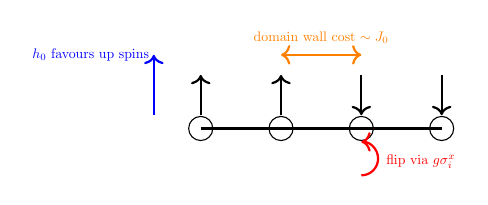
\begin{tikzpicture}[scale=0.85]
  \begin{scope}[yshift=-5cm]
    % chain
    \foreach \x in {0,1.2,2.4,3.6} {
      \draw[fill=white] (\x,0) circle (0.18);
    }
    \foreach \x/\y in {0/1.2,1.2/2.4,2.4/3.6} {
      \draw[thick] (\x,0) -- (\y,0);
    }

    % spins: two domains
    \draw[->,thick] (0,0.2) -- (0,0.8);
    \draw[->,thick] (1.2,0.2) -- (1.2,0.8);
    \draw[->,thick] (2.4,0.8) -- (2.4,0.2);
    \draw[->,thick] (3.6,0.8) -- (3.6,0.2);

    % mark domain wall
    \draw[thick,orange,<->] (1.2,1.1) -- (2.4,1.1);
    \node[orange,scale=0.5] at (1.8,1.35) {domain wall cost $\sim J_0$};

    % longitudinal field
    \draw[->,blue,thick] (-0.7,0.2) -- (-0.7,1.1);
    \node[blue,scale=0.5,anchor=east] at (-0.7,1.1) {$h_0$ favours up spins};

    % transverse flip arrow
    \draw[->,red,thick] (2.4,-0.7) arc (-90:90:0.25);
    \node[red,scale=0.5,anchor=west] at (2.7,-0.5) {flip via $g\sigma_i^x$};
  \end{scope}
\end{tikzpicture}
\end{figure}
\slidecitation{H.~Kim and D.~A.~Huse,
``Ballistic Spreading of Entanglement in a Diffusive Nonintegrable System'',
\textit{Physical Review Letters} (2013).}

\end{columns}

\end{frame}

%============== PART 5 – SLIDE 3 ==============

\begin{frame}{Floquet driving protocol in our model}


\small
\begin{itemize}
  \item Time-periodic Hamiltonian
  $
    H(t)=H_0(t)+H_1
  $
  \[
    H_0(t)=-J(t)\sum_{i}\sigma_i^z\sigma_{i+1}^z
            -h(t)\sum_i\sigma_i^z,
    \quad
    H_1=-g\sum_i\sigma_i^x
  \]
  \item Driving:
  $
    J(t),h(t)=
    \begin{cases}
    +J_0,+h_0,& 0\le t\le T/2\\
    -J_0,-h_0,& T/2<t\le T
    \end{cases}
  $
  \item Diagonal operators
  $
    \mathcal{O}_{zz}=\sum_{i}\sigma_i^z\sigma_{i+1}^z,\;
    \mathcal{O}_z=\sum_i\sigma_i^z,\;
    \mathcal{O}=J_0\mathcal{O}_{zz}+h_0\mathcal{O}_z
  $
  \item $[H_0(t),H_0(t')]=0$, $U_0(T,0)=\mathbb{I}$ (closed micromotion)
\end{itemize}

\centering
\begin{figure}
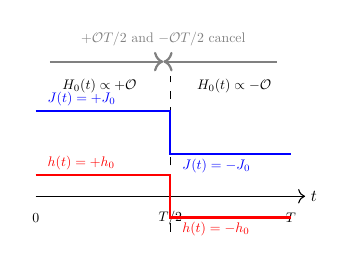
\begin{tikzpicture}[scale=0.9]
  % time axis
  \draw[->] (0,0) -- (3.8,0) node[right,scale=0.6] {$t$};
  \node[scale=0.5] at (0,-0.3) {$0$};
  \node[scale=0.5] at (1.9,-0.3) {$T/2$};
  \node[scale=0.5] at (3.6,-0.3) {$T$};
  \draw[dashed] (1.9,-0.5) -- (1.9,1.7);

  % J(t) square wave
  \draw[thick,blue]
    (0,1.2) -- (1.9,1.2) -- (1.9,0.6) -- (3.6,0.6);
  \node[blue,scale=0.5,anchor=south west] at (0.1,1.2) {$J(t)=+J_0$};
  \node[blue,scale=0.5,anchor=north west] at (2.0,0.6) {$J(t)=-J_0$};

  % h(t) square wave
  \draw[thick,red]
    (0,0.3) -- (1.9,0.3) -- (1.9,-0.3) -- (3.6,-0.3);
  \node[red,scale=0.5,anchor=south west] at (0.1,0.3) {$h(t)=+h_0$};
  \node[red,scale=0.5,anchor=north west] at (2.0,-0.3) {$h(t)=-h_0$};

  % labels +O and -O
  \node[scale=0.5] at (0.9,1.55) {$H_0(t)\propto +\mathcal{O}$};
  \node[scale=0.5] at (2.8,1.55) {$H_0(t)\propto -\mathcal{O}$};

  % net phase arrow
  \draw[->,thick,gray] (0.2,1.9) -- (1.8,1.9);
  \draw[->,thick,gray] (3.4,1.9) -- (1.8,1.9);
  \node[gray,scale=0.5,anchor=south] at (1.8,2.05) {$+\mathcal{O}T/2$ and $-\mathcal{O}T/2$ cancel};

\end{tikzpicture}

\end{figure}

Next show results.
\end{frame}

\section{Results}
\begin{frame}{Entanglement entropy plot in our model}
\small
Symmetric-square-wave periodic Hamiltonian, 
  $
    H(t)=H_0(t)+H_1
  $
  \[
    H_0(t)=-J(t)\sum_{i}\sigma_i^z\sigma_{i+1}^z
            -h(t)\sum_i\sigma_i^z,
    \quad
    H_1=-g\sum_i\sigma_i^x
  \]
\begin{figure}
    \centering
    \includegraphics[width=1.1\linewidth]{9th_sem_presentation/EE with TP.png}
    
    \label{EE with TP}
\end{figure}
    
\end{frame}

\begin{frame}{Autocorrelation in our model}
$$C_j(nT) = \langle \psi_0 | [\sigma^z_j(nT) ][\sigma^z_j(0) ] | \psi_0 \rangle $$
\begin{figure}
    \centering
    \includegraphics[width=1.09\linewidth]{9th_sem_presentation/Auto potential.png}
   
    \label{Auto potential}
\end{figure}
\end{frame}
\begin{frame}{Floquet Hamiltonian and prethermal fragmentation}


\small
\begin{columns}[T,onlytextwidth]

\column{0.52\textwidth}
\begin{itemize}\setlength\itemsep{3pt}
  \item Floquet unitary; effective Hamiltonian
  \[
    U_F(T) = \mathcal T e^{-i\int_0^T H(t)\,dt},
    \quad U_F = e^{-i H_F T}
  \]
  \item $(H_F^{(1)})_{nm}
=-\langle n|g\sum_{i=1}^{L}\sigma_i^x|m\rangle\,\left(\delta_{P_{nm},0}+(1-\delta_{P_{nm},0})
\operatorname{sinc}\!\Big(\frac{P_{nm}T}{4\hbar}\Big)e^{-\,\tfrac{i}{\hbar}P_{nm}\tfrac{T}{4}}\right)$ 
  constrained single-spin flips; almost block-diagonal in fragmented basis
  
  \item Tuning drive period \(T\) choose \(T\) so sinc-factors remove selected links; prethermal fragments
  
  \item Higher orders \(H_F^{(2)},H_F^{(3)},\dots\)
  weak off-diagonal couplings between fragments; slow late-time mixing
\end{itemize}

\column{0.48\textwidth}
\centering



\hspace{5cm}



\hspace{5cm}





\hspace{5cm}


\hspace{5cm}



\hspace{5cm}


\hspace{5cm}


\hspace{5cm}



\hspace{5cm}
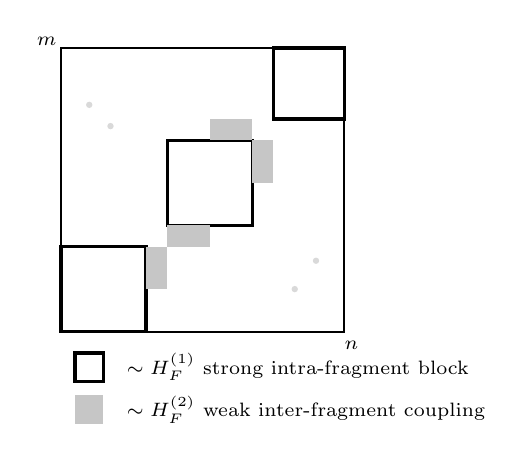
\begin{tikzpicture}[scale=0.9]

  % full matrix
  \draw[thick] (0,0) rectangle (4,4);
  \node[font=\scriptsize] at (4.1,-0.2) {$n$};
  \node[font=\scriptsize] at (-0.2,4.1) {$m$};

  % strong diagonal blocks ~ H_F^{(1)}
  \draw[very thick] (0,0) rectangle (1.2,1.2);
  \draw[very thick] (1.5,1.5) rectangle (2.7,2.7);
  \draw[very thick] (3.0,3.0) rectangle (4.0,4.0);

  % weak second-order couplings near blocks
  \fill[gray!45] (1.2,0.6) rectangle (1.5,1.2);   % between block 1 and 2
  \fill[gray!45] (1.5,1.2) rectangle (2.1,1.5);

  \fill[gray!45] (2.7,2.1) rectangle (3.0,2.7);   % between block 2 and 3
  \fill[gray!45] (2.1,2.7) rectangle (2.7,3.0);

  % a few tiny remote off-diagonal elements
  \foreach \p in {(0.4,3.2),(0.7,2.9),(3.3,0.6),(3.6,1.0)}{
    \fill[gray!30] \p circle (0.045);
  }

  % legend
  \draw[very thick] (0.2,-0.7) rectangle (0.6,-0.3);
  \node[font=\scriptsize,anchor=west] at (0.7,-0.5)
    {$\;\sim H_F^{(1)}$ strong intra-fragment block};

  \fill[gray!45] (0.2,-1.3) rectangle (0.6,-0.9);
  \node[font=\scriptsize,anchor=west] at (0.7,-1.1)
    {$\;\sim H_F^{(2)}$ weak inter-fragment coupling};

\end{tikzpicture}

\end{columns}
\end{frame}


\begin{frame}{Bulk $P_{nm}$ values for states connected by $\sum_{i=1}^{L}\sigma_i^x$}
Take  $J_0=h_0/2$
\small
\begin{figure}[!htb]
\centering
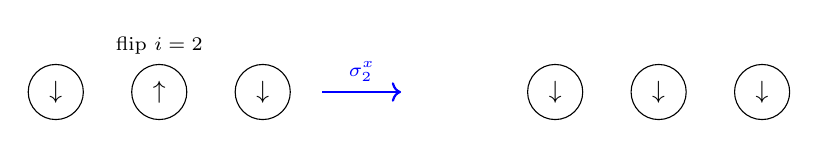
\begin{tikzpicture}
  \node[spin] (L) {$\downarrow$};
  \node[spin, right=6mm of L, label=above:{\scriptsize flip $i=2$}] (M) {$\uparrow$};
  \node[spin, right=6mm of M] (R) {$\downarrow$};
  \draw[fliparrow] ($(R.east)+(4mm,0)$) -- ++(10mm,0)
      node[midway, above] {\scriptsize $\sigma_2^x$};
  \node[spin, right=30mm of R] (L2) {$\downarrow$};
  \node[spin, right=6mm of L2] (M2) {$\downarrow$};
  \node[spin, right=6mm of M2] (R2) {$\downarrow$};
\end{tikzpicture}
\caption{$P_{nm}=0$}
\end{figure}

\begin{figure}[!htb]
\centering
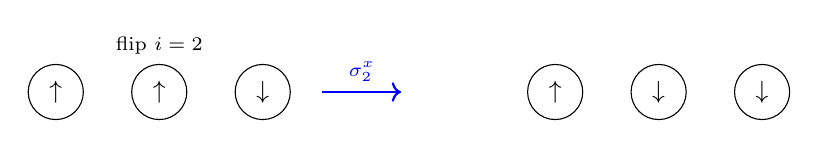
\begin{tikzpicture}
  \node[spin] (L) {$\uparrow$};
  \node[spin, right=6mm of L, label=above:{\scriptsize flip $i=2$}] (M) {$\uparrow$};
  \node[spin, right=6mm of M] (R) {$\downarrow$};
  \draw[fliparrow] ($(R.east)+(4mm,0)$) -- ++(10mm,0)
      node[midway, above] {\scriptsize $\sigma_2^x$};
  \node[spin, right=30mm of R] (L2) {$\uparrow$};
  \node[spin, right=6mm of L2] (M2) {$\downarrow$};
  \node[spin, right=6mm of M2] (R2) {$\downarrow$};
\end{tikzpicture}
\caption{$P_{nm}=-4 J_0$}
\end{figure}

\begin{figure}[!htb]
\centering
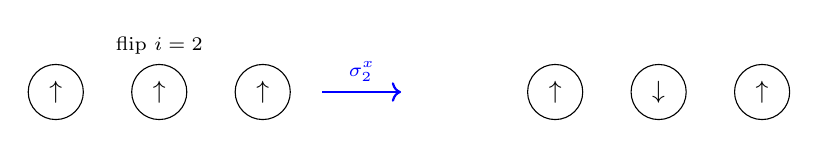
\begin{tikzpicture}
  \node[spin] (L) {$\uparrow$};
  \node[spin, right=6mm of L, label=above:{\scriptsize flip $i=2$}] (M) {$\uparrow$};
  \node[spin, right=6mm of M] (R) {$\uparrow$};
  \draw[fliparrow] ($(R.east)+(4mm,0)$) -- ++(10mm,0)
      node[midway, above] {\scriptsize $\sigma_2^x$};
  \node[spin, right=30mm of R] (L2) {$\uparrow$};
  \node[spin, right=6mm of L2] (M2) {$\downarrow$};
  \node[spin, right=6mm of M2] (R2) {$\uparrow$};
\end{tikzpicture}
\caption{$P_{nm}=-8 J_0$}
\end{figure}
\end{frame}

\begin{frame}{Edge $P_{nm}$ values for states connected by $H_1$}
 For open boundary conditions, additional edge processes occur:

\begin{figure}[!htb]
\centering
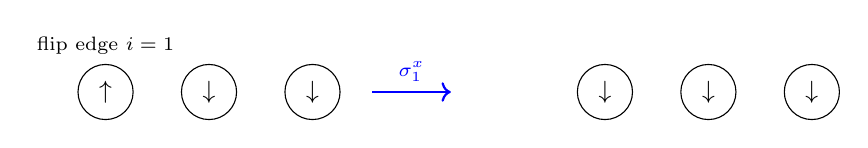
\begin{tikzpicture}
  \node[spin, label=above:{\scriptsize flip edge $i=1$}] (L) {$\uparrow$};
  \node[spin, right=6mm of L] (M) {$\downarrow$};
  \node[spin, right=6mm of M] (R) {$\downarrow$};
  \draw[fliparrow] ($(R.east)+(4mm,0)$) -- ++(10mm,0)
      node[midway, above] {\scriptsize $\sigma_1^x$};
  \node[spin, right=30mm of R] (L2) {$\downarrow$};
  \node[spin, right=6mm of L2] (M2) {$\downarrow$};
  \node[spin, right=6mm of M2] (R2) {$\downarrow$};
\end{tikzpicture}
\caption{$P_{nm}=-2 J_0$}
\end{figure}

\begin{figure}[!htb]
\centering
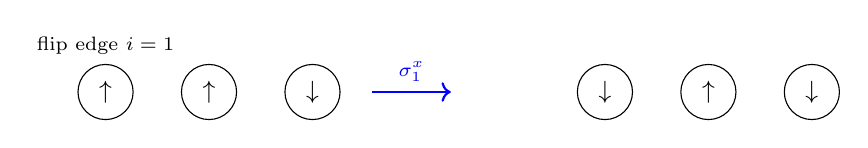
\begin{tikzpicture}
  \node[spin, label=above:{\scriptsize flip edge $i=1$}] (L) {$\uparrow$};
  \node[spin, right=6mm of L] (M) {$\uparrow$};
  \node[spin, right=6mm of M] (R) {$\downarrow$};
  \draw[fliparrow] ($(R.east)+(4mm,0)$) -- ++(10mm,0)
      node[midway, above] {\scriptsize $\sigma_1^x$};
  \node[spin, right=30mm of R] (L2) {$\downarrow$};
  \node[spin, right=6mm of L2] (M2) {$\uparrow$};
  \node[spin, right=6mm of M2] (R2) {$\downarrow$};
\end{tikzpicture}
\caption{$P_{nm}=-6 J_0$}
\end{figure}


From the different driving, we can fix all spin flips other than $P_{nm}=0$. In this case we see that blocks of $\uparrow$ in states do not change. This is our local conserved quantity. 
\end{frame}
\begin{frame}{Time period of drive and allowed transitions in periodic boundary conditions}
$(H_F^{(1)})_{nm}
=-\langle n|g\sum_{i=1}^{L}\sigma_i^x|m\rangle\,\left(\delta_{P_{nm},0}+(1-\delta_{P_{nm},0})
\operatorname{sinc}\!\Big(\frac{P_{nm}T}{4\hbar}\Big)e^{-\,\tfrac{i}{\hbar}P_{nm}\tfrac{T}{4}}\right)$ 
\begin{table}[!htb]
\centering
\caption{First-order (single flip) connectivity for PBC at $h_0 = 2J_0$. 
Parentheses indicate $PT/4$.}

\begin{tabular}{|c|c|c|c|}
\hline
$T$ & $P = 0$ & $P = 4J_0$ & $P = 8J_0$ \\
\hline
$\tfrac{\pi}{2J_0}$ & on $(0)$ 
& on $(\tfrac{\pi}{2})$ 
& off $(\pi)$ \\
\hline
$\tfrac{\pi}{J_0}$ & on $(0)$ 
& off $(\pi)$ 
& off $(2\pi)$ \\
\hline
\end{tabular}

\vspace{0.6em}
\small
\label{Tab:PBC}
\end{table}
\end{frame}
\begin{frame}{Time period of drive and allowed transitions in open boundary conditions}
$(H_F^{(1)})_{nm}
=-\langle n|g\sum_{i=1}^{L}\sigma_i^x|m\rangle\,\left(\delta_{P_{nm},0}+(1-\delta_{P_{nm},0})
\operatorname{sinc}\!\Big(\frac{P_{nm}T}{4\hbar}\Big)e^{-\,\tfrac{i}{\hbar}P_{nm}\tfrac{T}{4}}\right)$   

\begin{table}[!htb]
\centering
\caption{First-order (single flip) connectivity for OBC at $h_0 = 2J_0$ (including edge flips). 
Parentheses indicate $PT/4$.}
\resizebox{\linewidth}{!}{%
\begin{tabular}{|c|c|c|c|c|c|c|}
\hline
$T$ & $P=0$ & $P=2J_0$ (edge) & $P=4J_0$ & $P=6J_0$ (edge) & $P=8J_0$ & Summary \\
\hline
$\tfrac{\pi}{2J_0}$ 
& on $(0)$ 
& on $(\tfrac{\pi}{4})$ 
& on $(\tfrac{\pi}{2})$ 
& on $(\tfrac{3\pi}{4})$ 
& off $(\pi)$ 
& only $|P|=8J_0$ killed \\
\hline
$\tfrac{\pi}{J_0}$ 
& on $(0)$ 
& on $(\tfrac{\pi}{2})$ 
& off $(\pi)$ 
& on $(\tfrac{3\pi}{2})$ 
& off $(2\pi)$ 
& kills $|P|=4,8$ \\
\hline
$\tfrac{2\pi}{J_0}$ 
& on $(0)$ 
& off $(\pi)$ 
& off $(2\pi)$ 
& off $(3\pi)$ 
& off $(4\pi)$ 
& all nonzero $P$ killed \\
\hline
\end{tabular}}

\vspace{0.6em}
\small
\label{Tab:OBC}
\end{table}

\end{frame}
\begin{frame}{Autocorrelation in open chain at different sites I}
The time period is $T=\pi/J_0$.
    \begin{figure}
        \centering
        \includegraphics[width=1.09\linewidth]{T1SiteAutocorrelationOpen.png}

        \label{T1SiteAutocorrelationOpen}
    \end{figure}
\end{frame}    

\begin{frame}{Autocorrelation in open chain at different sites II}

The time period is $T=2\pi/J_0$.
\begin{figure}
    \centering
    \includegraphics[width=1.09\linewidth]{T2SiteAutocorrelationOpen.png}

    \label{T2SiteAutocorrelationOpen}
\end{figure}

\end{frame}
\section{Conclusion}
\begin{frame}{Summary: first-order Floquet selection and fragmentation}

\small
\begin{columns}[T,onlytextwidth]

\column{0.55\textwidth}
\begin{itemize}\setlength\itemsep{2pt}
  \item Drive, basis:\\
        TLFIM, symmetric sign flip; $h_0=2J_0$; diagonal $\mathcal O$ in $\sigma^z$ basis
  \item Floquet selection: $P_{nm}=0$ flips
  \item Matrix elements $\sigma_i^x$ follow bulk three-site rule; extra edge flips violate it at $T=\pi/J_0$
  \item Conserved quantities:
        $I_i=n_i^\uparrow n_{i+1}^\uparrow$; 
  \item Fragmentation, heating:\\
        frozen $\uparrow\uparrow$ domains; heating confined within each fragment
\end{itemize}

\vspace{1mm}
\[
 (H_F^{(1)})_{nm}
 =(H_1)_{nm}\,
 \mathrm{sinc}\!\Big(\tfrac{P_{nm}T}{4}\Big)
 e^{-iP_{nm}T/4},
 \quad
 H_1=-g\sum_i\sigma_i^x
\]
\[
 I_i=n_i^\uparrow n_{i+1}^\uparrow,\quad
 n_i^\uparrow=\tfrac12(1+\sigma_i^z)
\]

\column{0.45\textwidth}
\centering
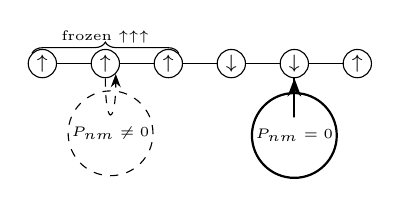
\begin{tikzpicture}[scale=0.8,>=Stealth,
  every node/.style={circle,draw,inner sep=1pt,font=\scriptsize}]
  \node (s1) at (0,0) {$\uparrow$};
  \node (s2) at (1,0) {$\uparrow$};
  \node (s3) at (2,0) {$\uparrow$};
  \node (s4) at (3,0) {$\downarrow$};
  \node (s5) at (4,0) {$\downarrow$};
  \node (s6) at (5,0) {$\uparrow$};

  \foreach \a/\b in {s1/s2,s2/s3,s3/s4,s4/s5,s5/s6} {
    \draw (\a) -- (\b);
  }

  % Override node style here!
  \draw[decorate,decoration={brace,amplitude=4pt}]
    (s1.north west) -- (s3.north east)
    node[midway,yshift=6pt,draw=none,rectangle,inner sep=1pt,font=\tiny]{frozen $\uparrow\uparrow\uparrow$};

  \draw[->,thick]
    (s5.south) .. controls +(0,-0.8) and +(0,-0.8) .. (s5.south)
    node[midway,yshift=-7pt,font=\tiny]{$P_{nm}=0$};

  \draw[->,dashed]
    (s2.south) .. controls +(0,-0.8) and +(0,-0.8) .. (s2.south east)
    node[midway,yshift=-7pt,font=\tiny]{$P_{nm}\neq0$};
\end{tikzpicture}


\vspace{1mm}
{\scriptsize Resonant (solid) vs blocked (dashed) flips}

\end{columns}
\end{frame}
\begin{frame}{Future directions}

\small
\begin{itemize}\setlength\itemsep{3pt}
  \item Graph-theoretic analysis of $H_F$ connectivity vs $T$, $g/J_0$, $L$; invariant components, sector dimensions
  \item Entanglement saturation vs fragment Page values; entanglement-based confirmation of fragmentation
  \item Symmetry structure and edge modes of Floquet spectrum; bulk–edge contrast in autocorrelation plateaus
  \item Higher-order Floquet corrections, larger $L$; distinguish true fragmentation vs prethermal plateaus; robustness in thermodynamic limit
  \item Search for explicit emergent conserved quantities enabling Floquet-engineered constrained dynamics
\end{itemize}

\end{frame}


{\setbeamercolor{palette primary}{fg=black, bg=yellow}
\begin{frame}[standout]
  Questions?
\end{frame}
}
\section{ETH backup slides}
\begin{frame}{Random matrix theory picture: operator matrix elements}

\begin{columns}[T,onlytextwidth]

\column{0.55\textwidth}
\small
\begin{itemize}
  \item Simple basis $\{\ket{i}\}_{i=1}^{\mathcal D}$: $\hat O$ diagonal
  \[
    \hat O = \sum_i O_i \ket{i}\!\bra{i}
  \]
  \item Chaotic eigenstates of $\hat H$:
  \[
    \psi_i^m := \braket{i|E_m},\quad
    \ket{E_m} = \sum_i \psi_i^m \ket{i}
  \]
  \item Operator in energy basis:
  \[
    O_{mn} = \matrixel{E_m}{\hat O}{E_n}
           = \sum_i O_i (\psi_i^m)^\ast \psi_i^n
  \]
  \item RMT eigenvectors: random orthogonal
  \[
    \overline{(\psi_i^m)^\ast \psi_j^n}
    = \frac{1}{\mathcal D}\delta_{mn}\delta_{ij}
  \]

\end{itemize}

\column{0.45\textwidth}
\centering
\begin{figure}
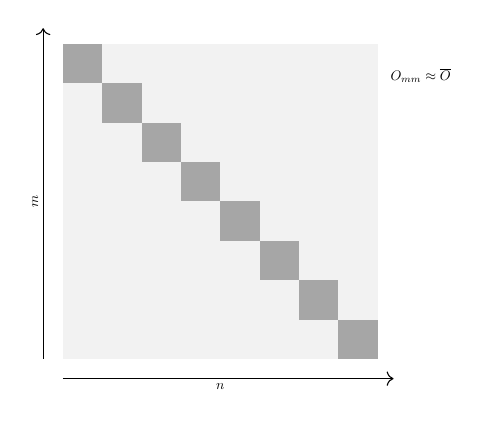
\begin{tikzpicture}[scale=0.5]
  % matrix grid
  \foreach \i in {0,...,7} {
    \foreach \j in {0,...,7} {
      \pgfmathsetmacro{\shade}{ifthenelse(\i==\j,70,10)}
      \fill[gray!\shade] (\i,7-\j) rectangle (\i+1,8-\j);
    }
  }
  % axes labels
  \draw[->] (-0.5,0) -- (-0.5,8.4);
  \node[rotate=90,anchor=south,scale=0.5] at (-0.5,4) {$m$};
  \draw[->] (0,-0.5) -- (8.4,-0.5);
  \node[anchor=north,scale=0.5] at (4,-0.5) {$n$};
  % diagonal label
  \node[scale=0.5,anchor=west] at (8.2,7.2) {$O_{mm}\approx\overline O$};
\end{tikzpicture}

\caption{\scriptsize Diagonal-dominated operator matrix in chaotic energy basis; RMT cartoon of ETH structure.}
\end{figure}
References: Srednicki~\cite{srednicki_chaos_1994}
\end{columns}
\end{frame}

%========= RMT SLIDE 2 =========
\begin{frame}{Random Matrix Theory picture: fluctuations and ETH-like structure}

\begin{columns}[T,onlytextwidth]

\column{0.55\textwidth}
\small
\begin{itemize}
  \item Averages:
  \[
    \overline{O_{mm}} = \overline{O},
    \quad
    \overline{O_{mn}} = 0\ (m\neq n)
  \]
  \item Off-diagonal variance
  \[
    \overline{|O_{mn}|^2}
    = \frac{1}{\mathcal D}\,\overline{O^2},
    \quad m\neq n
  \]
  \item ETH-like structure
  \[
    O_{mn}
    \approx \overline{O}\,\delta_{mn}
      + \sqrt{\frac{\overline{O^2}}{\mathcal D}}\;R_{mn}
  \]
  \item Scaling:
        $|O_{mn}|\sim \mathcal D^{-1/2}
        \sim e^{-S/2}$
\end{itemize}

\column{0.45\textwidth}
\centering
\begin{figure}
\begin{tikzpicture}[scale=0.5]
  % matrix grid with noisy off-diagonals
  \foreach \i in {0,...,7} {
    \foreach \j in {0,...,7} {
      \pgfmathsetmacro{\shade}{
        ifthenelse(\i==\j,70,5+10*rand)
      }
      \fill[gray!\shade] (\i,7-\j) rectangle (\i+1,8-\j);
    }
  }
  % draw matrix border more visibly
  \draw[black,thick] (0,0) rectangle (8,8);

  % annotate diagonal: keep start/end inside
  \draw[red,thick] (0.05,7.95) -- (7.95,0.05);

  % annotation nodes inside or just out of border
  \node[red,scale=0.7,anchor=west] at (1,7.7) {smooth diagonals};
  \node[blue,scale=0.7,anchor=west] at (3.5,5.5) {small random off-diagonals};
\end{tikzpicture}


\caption{\scriptsize Operator matrix in chaotic basis: almost-constant diagonal band plus $\mathcal D^{-1/2}$-scaled random off-diagonals; random-matrix ETH cartoon .}
\end{figure}
References: Srednicki~\cite{srednicki_chaos_1994}
\end{columns}
\end{frame}

\begin{frame}{Off-diagonal ETH and small fluctuations}
Backup
\begin{columns}[T,onlytextwidth]

\column{0.55\textwidth}
\small
\begin{itemize}
  \item Fluctuations around plateau:
  \[
    \delta A(t)
    = \langle A\rangle(t) - \overline{\langle A\rangle}
    = \sum_{m\neq n} C_m^\ast C_n
      e^{i(E_m-E_n)t} A_{mn}
  \]
  \item Time-averaged variance:
  \[
    \overline{\delta A^2}
    = \sum_{m\neq n}
      |C_m|^2 |C_n|^2 |A_{mn}|^2
  \]
  \item ETH off-diagonals:
        $|A_{mn}|^2 \sim e^{-S(\bar E)}$
  \item Narrow shell; bounded $f_A$, $R_{mn}$; sum of weights $\le 1$
  \item Result:
        $\overline{\delta A^2}\lesssim e^{-S(\bar E)}\sim e^{-cL}$;
        fluctuations exponentially small
\end{itemize}

\column{0.45\textwidth}
\centering
\begin{figure}
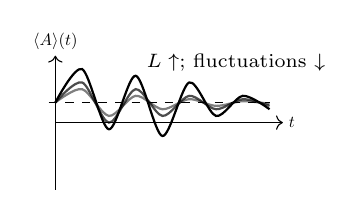
\begin{tikzpicture}[scale=0.85]

  % axes
  \draw[->] (0,0) -- (3.4,0) node[right,scale=0.6] {$t$};
  \draw[->] (0,-1.0) -- (0,1.0) node[above,scale=0.6] {$\langle A\rangle(t)$};

  % plateau line
  \draw[dashed] (-0.1,0.3) -- (3.2,0.3);

  % L=8
  \draw[thick]
    plot[smooth] coordinates {
      (0,0.3) (0.4,0.8) (0.8,-0.1)
      (1.2,0.7) (1.6,-0.2) (2.0,0.6)
      (2.4,0.1) (2.8,0.4) (3.2,0.2)
    };

  % L=10 (smaller amplitude)
  \draw[thick,opacity=0.7]
    plot[smooth] coordinates {
      (0,0.3) (0.4,0.6) (0.8,0.0)
      (1.2,0.5) (1.6,0.1) (2.0,0.4)
      (2.4,0.2) (2.8,0.35) (3.2,0.25)
    };

  % L=12 (even smaller)
  \draw[thick,opacity=0.5]
    plot[smooth] coordinates {
      (0,0.3) (0.4,0.5) (0.8,0.1)
      (1.2,0.4) (1.6,0.2) (2.0,0.35)
      (2.4,0.25) (2.8,0.32) (3.2,0.28)
    };

  \node[font=\scriptsize] at (2.7,0.9) {$L\uparrow$; fluctuations $\downarrow$};

\end{tikzpicture}
\caption{\scriptsize Off-diagonal ETH $\rightarrow$ exponentially small temporal fluctuations; larger systems look more “thermal” in time.\\
D’Alessio et al.\ (2016)~\cite{dalessio_quantum_2016}.}
\end{figure}

\end{columns}
\end{frame}
\begin{frame}{ETH ansatz: energy and locality}

\begin{columns}[T,onlytextwidth]

\column{0.55\textwidth}
\small
\begin{itemize}
  \item Nonintegrable, ``quantum chaotic'' lattice system
  \item ETH ansatz for few-body $A$:
  \[
    A_{mn}
    = A(\bar E)\,\delta_{mn}
      + e^{-S(\bar E)/2} f_A(\bar E,\omega)\,R_{mn}
  \]
  \item Mean energy
        $\bar E=(E_m+E_n)/2$;
        frequency $\omega=E_n-E_m$
  \item $A(\bar E)$: smooth microcanonical value
  \item $S(\bar E)$: thermodynamic entropy $\sim s(\bar e)L$
  \item $R_{mn}$: random, zero mean, unit variance
\end{itemize}

\column{0.45\textwidth}
\centering
\begin{figure}
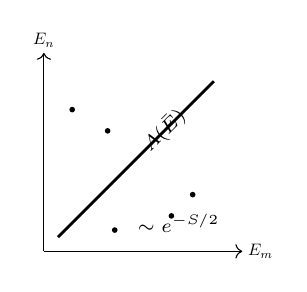
\begin{tikzpicture}[scale=0.9]

  % axes
  \draw[->] (0,0) -- (2.8,0) node[right,scale=0.6] {$E_m$};
  \draw[->] (0,0) -- (0,2.8) node[above,scale=0.6] {$E_n$};

  % diagonal ETH band
  \draw[line width=1pt] (0.2,0.2) -- (2.4,2.4);
  \node[font=\scriptsize,rotate=45] at (1.7,1.7) {$A(\bar E)$};

  % off-diagonal random speckles
  \foreach \p in {{(0.4,2.0)}, {(1.0,0.3)}, {(2.1,0.8)}, {(0.9,1.7)}, {(1.8,0.5)}} {
    \fill \p circle (0.04);
  }

  \node[font=\scriptsize] at (1.9,0.4) {$\sim e^{-S/2}$};
\end{tikzpicture}

\caption{\scriptsize ETH structure: smooth diagonals, entropy-suppressed random off-diagonals.}
\end{figure}
References:
Deutsch (1991)~\cite{deutsch_quantum_1991}, Srednicki (1994)~\cite{srednicki_chaos_1994}, D’Alessio et al.\ (2016)~\cite{dalessio_quantum_2016}
\end{columns}

\end{frame}
\section{ETH violation backup}
\begin{frame}{Entanglement entropy as ETH diagnostic}
Backup
\begin{columns}[T,onlytextwidth]

\column{0.55\textwidth}
\small
\begin{itemize}
  \item Bipartition: $\mathcal{H}=\mathcal{H}_A\otimes\mathcal{H}_B$;\\
        $\dim\mathcal{H}_A=d_A$, $\dim\mathcal{H}_B=d_B$
  \item Eigenstate reduced state:\\
        $\rho_A^{(\alpha)}=\Tr_B\dyad{E_\alpha}$
  \item Entanglement entropy:\\
        $S_A(\alpha)=-\Tr_A\!\big[\rho_A^{(\alpha)}\log\rho_A^{(\alpha)}\big]$
  \item ETH expectation:
        $\rho_A^{(\alpha)}\approx\rho_A^{\mathrm{th}}(e)$,\\
        $S_A(\alpha)\approx S_A^{\mathrm{th}}(e)\simeq s(e)\,|A|$
  \item Random / Page behaviour:\\
        $S_A^{\mathrm{Page}}\simeq\log d_A-\dfrac{d_A}{2d_B}$
  \item Diagnostic: finite fraction with\\
        $S_A(\alpha)\le S_A^{\mathrm{th}}(e)-\delta|A|$;\\
        one-to-one map of entropy, $\Rightarrow$ there is finite trace distance\\
        $\rho_A^{(\alpha)}\ne\rho_A^{\mathrm{th}}(e)$; ETH breakdown
\end{itemize}

\column{0.45\textwidth}
\centering
\begin{figure}
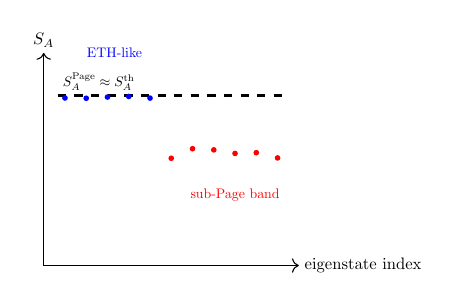
\begin{tikzpicture}[scale=0.9]
  % axes
  \draw[->] (0,0) -- (3.6,0) node[right,scale=0.6] {eigenstate index};
  \draw[->] (0,0) -- (0,3.0) node[above,scale=0.6] {$S_A$};

  % Page / thermal line
  \draw[dashed,thick] (0.2,2.4) -- (3.4,2.4);
  \node[scale=0.5,anchor=south west] at (0.2,2.4) {$S_A^{\mathrm{Page}}\approx S_A^{\mathrm{th}}$};

  % ETH-like points near Page line
  \foreach \x in {0.3,0.6,0.9,1.2,1.5} {
    \fill[blue] (\x,2.35+0.05*rnd) circle (0.04);
  }

  % fragmented / non-ETH band
  \foreach \x in {1.8,2.1,2.4,2.7,3.0,3.3} {
    \fill[red] (\x,1.4+0.25*rnd) circle (0.04);
  }

  % label regions
  \node[scale=0.5,blue] at (1.0,3) {ETH-like};
  \node[scale=0.5,red]  at (2.7,1.0) {sub-Page band};
\end{tikzpicture}
\caption{\scriptsize Eigenstate entanglement entropy; Page / thermal line versus sub-Page band.}
\end{figure}
References: \\
Page 1993~\cite{page_average_1993}; \\Foong \& Kanno 1994~\cite{foong_proof_1994};\\
Ghosh–Paul–Sengupta  2023~\cite{ghosh_prethermal_2023}.
\end{columns}

\end{frame}
%========== PART 4 – SLIDE 1: ENTANGLEMENT ENTROPY ==========



%========== PART 4 – SLIDE 2: AUTOCORRELATIONS ==========

\begin{frame}{Infinite-temperature autocorrelations as ETH diagnostic}

\begin{columns}[T,onlytextwidth]

\column{0.55\textwidth}
\small
\begin{itemize}
  \item Static $H$; local $A$; Hilbert dimension $D$
  \item Infinite-$T$ autocorrelation:\\
        $C_A(t)=\dfrac{1}{D}\Tr[A(t)A(0)]$,\\
        $A(t)=e^{iHt}Ae^{-iHt}$
  \item Long-time limit (nondegenerate gaps):
        $C_A^\infty=\dfrac{1}{D}\sum_n |A_{nn}|^2$
  \item ETH scaling (traceless, charge-orthogonal $A$):
        $|A_{nn}|^2\sim e^{-S(E)}$;\\
        $C_A^\infty\sim e^{-cL}\rightarrow 0$
  \item Mazur projection onto conserved $\{Q_k\}$:\\
        $A_\parallel=\sum_{k,\ell}(A,Q_k)[C^{-1}]_{k\ell}Q_\ell$\\
        $C_A^\infty\ge D_A=\dfrac{1}{D}\Tr(A_\parallel^\dagger A_\parallel)$
  \item Fragmentation: conserved projectors $P_\alpha$;
        finite $A_\parallel$; nonvanishing $C_A^\infty$ plateau
\end{itemize}

\column{0.45\textwidth}
\centering
\begin{figure}
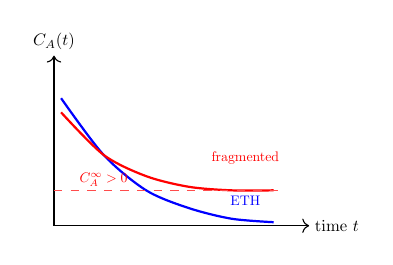
\begin{tikzpicture}[scale=0.9]
  % axes
  \draw[->] (0,0) -- (3.6,0) node[right,scale=0.6] {time $t$};
  \draw[->] (0,0) -- (0,2.4) node[above,scale=0.6] {$C_A(t)$};

  % ETH-like decay
  \draw[thick,blue,smooth]
    plot coordinates {(0.1,1.8) (0.7,1.0) (1.3,0.5) (1.9,0.25) (2.5,0.1) (3.1,0.05)};
  \node[scale=0.5,blue] at (2.7,0.35) {ETH};

  % fragmented plateau
  \draw[thick,red,smooth]
    plot coordinates {(0.1,1.6) (0.7,1.0) (1.3,0.7) (1.9,0.55) (2.5,0.5) (3.1,0.5)};
  \node[scale=0.5,red] at (2.7,0.95) {fragmented};

  % plateau line
  \draw[dashed,red!70] (0.0,0.5) -- (3.2,0.5);
  \node[scale=0.5,red] at (0.7,0.65) {$C_A^\infty>0$};
\end{tikzpicture}
\caption{\scriptsize Infinite-$T$ autocorrelations; ETH decay versus nonzero plateau from conserved components.
}
\end{figure}
References:\\
Mazur 1969~\cite{mazur_non-ergodicity_1969};\\
Nandkishore \& Huse 2015~\cite{nandkishore_many-body_2015};\\
Sala et al.\ 2020~\cite{sala_ergodicity_2020};\\
Ghosh–Paul–Sengupta \ 2023 ~\cite{ghosh_prethermal_2023}.
\end{columns}

\end{frame}




\section{Spin 1/2 chain backup} 
\begin{frame}{Spin-$\tfrac12$ Ising chain: microscopic playground}
\small
\begin{itemize}
  \item Static Hamiltonian
  \[
    H_{\mathrm{stat}}
    = - J_0 \sum_{i=1}^{L-1} \sigma_i^z \sigma_{i+1}^z
      - h_0 \sum_{i=1}^{L} \sigma_i^z
      - g \sum_{i=1}^L \sigma_i^x,
      \; |g|\ll|J_0|,|h_0|
  \]
  \item Minimal quantum lattice model for magnetism and quantum phase transitions
  \item Sites $i=1,\dots,L$; local space $\mathcal{H}_i \cong \mathbb{C}^2$, Total space $\mathcal{H}=\bigotimes_{i=1}^L \mathcal{H}_i$, $\dim\mathcal{H}=2^L$
  \item Computational basis: $\sigma^z$ eigenstates $\{\ket{\uparrow}_i,\ket{\downarrow}_i\}$, Product states $\ket{s_1\cdots s_L}$ as classical spin configurations $\sigma_i^z$: local magnetisation; $\sigma_i^x$: single-spin flip, quantum fluctuations
\end{itemize}
\centering
\begin{figure}
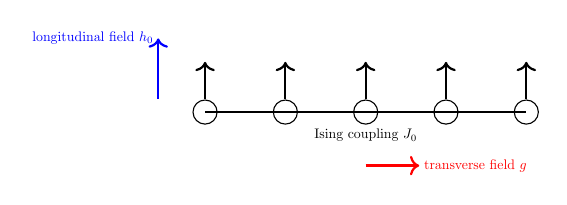
\begin{tikzpicture}[scale=0.85]
  % sites
  \foreach \x in {0,1.2,2.4,3.6,4.8} {
    \draw[fill=white] (\x,0) circle (0.18);
  }
  % bonds J0
  \foreach \x/\y in {0/1.2,1.2/2.4,2.4/3.6,3.6/4.8} {
    \draw[thick] (\x,0) -- (\y,0);
  }
  \node[scale=0.5] at (2.4,-0.35) {Ising coupling $J_0$};

  % local z-arrows (spins)
  \foreach \x in {0,1.2,2.4,3.6,4.8} {
    \draw[->,thick] (\x,0.2) -- (\x,0.75);
  }

  % longitudinal field h0
  \draw[->,thick,blue] (-0.7,0.2) -- (-0.7,1.1);
  \node[blue,scale=0.5,anchor=east] at (-0.7,1.1) {longitudinal field $h_0$};

  % transverse field g
  \draw[->,thick,red] (2.4,-0.8) -- (3.2,-0.8);
  \node[red,scale=0.5,anchor=west] at (3.2,-0.8) {transverse field $g$};
\end{tikzpicture}
\caption{\scriptsize Spin-$\tfrac12$ chain with nearest-neighbour Ising coupling and longitudinal / transverse fields.}
\end{figure}
\end{frame}

\section{Floquet perturbation theory}
\begin{frame}{Floquet perturbation theory and first-order $H_F^{(1)}$}

\begin{columns}[T,onlytextwidth]

% ------- LEFT: general Floquet perturbation theory -------
\column{0.48\textwidth}
\small

\textbf{Interaction picture; first-order $H_F$}
\begin{itemize}\setlength\itemsep{2pt}
  \item Split Hamiltonian:
  \[
    H(t)=H_0(t)+V
  \]
  \item Interaction picture:
  \[
    U^I(t,0)=U_0(0,t)\,U(t,0)
  \]
  \[
    V_I(t)=U_0(0,t)\,V\,U_0(t,0)
  \]
   \[
    i\hbar\,\partial_t U^I(t,0)=V_I(t)\,U^I(t,0)
  \]
  \item One-period Floquet operator:
  \[
    U(T,0)=U_0(T,0)\,U^I(T,0)
  \]
  \item If $U_0(T,0)=\mathbb{I}$:
  \[
    U(T,0)=U^I(T,0)
    =e^{-\,\frac{i}{\hbar}H_F T}
  \]
\end{itemize}

% ------- RIGHT: our driven Ising chain -------
\column{0.52\textwidth}
\small
\begin{itemize} 
  \item First-order Floquet Hamiltonian:
  \[
    H_F^{(1)}
    =\frac{1}{T}\int_0^T\!dt\,V_I(t)
  \]
\end{itemize}
\textbf{Application:  Ising drive}
\begin{itemize}\setlength\itemsep{2pt}
  \item Symmetric square wave $J(t),h(t)$:
  \[
    [H_0(t),H_0(t')]=0,\quad U_0(T,0)=\mathbb{I}
  \]
  \item $\mathcal O$–eigenbasis:
  $
    \mathcal O\ket{m}=P_m\ket{m},\quad P_{nm}=P_n-P_m
 $
  \item First-order matrix element:
  $(H_F^{(1)})_{nm}=-\Big\langle n\big|g\sum_{i=1}^{L}\sigma_i^x\big|m\Big\rangle$\\$\left[
\delta_{P_{nm},0}+(1-\delta_{P_{nm},0})
\operatorname{sinc}\!\Big(\frac{P_{nm}T}{4\hbar}\Big)e^{-\,\tfrac{i}{\hbar}P_{nm}\tfrac{T}{4}}\right].
$
\item Find T so that $sinc$ term vanishes and take $J_0=h_0/2$
\end{itemize}


\end{columns}

\end{frame}

\end{document}
